\section{Застосування розробленого ПЗ}
\subsection{Вхідна та вихідна інформація}

Для тестування розробленого ПЗ була використана модель маркетингового каналу, яка зображена на рис. \ref{fig:real_channel}. До неї входять наступні гравці: один виробник, два дистриб’ютори, чотири рітейлери, шість клієнтів. Всі гравці, окрім єдиного виробника, є автоматичними, а рішення виробника приймає користувач системи.

\begin{stdfigure}
    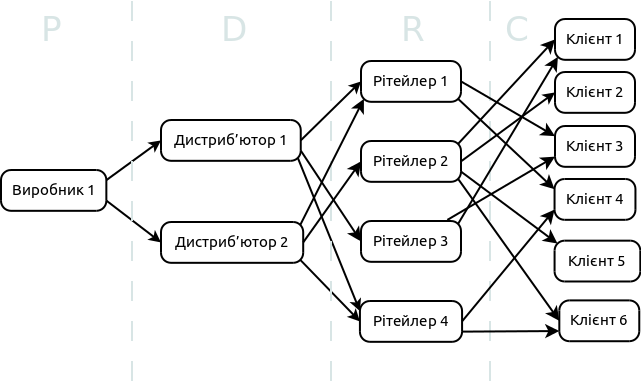
\includegraphics[width=5in]{images/real_channel.png}
    \caption{Модель каналу, що була використана для тестування ПЗ}
    \label{fig:real_channel}
\end{stdfigure}

В ході тестування було виконано три ігрових ітерації, в рамках яких було виконано 72 ходи. На третій ітерації виробник не зміг обслугувати вхідні замовлення і гра була зупинена. Були отримані наступні результати:
\begin{longEnumerate}
\item Станом на перший хід, гравці мали наступні запаси: виробники --- 10 одиниць, клієнти --- 135 одиниць, дистриб’ютори --- 6 одиниць, рітейлери --- 19 одиниць. Після другого ходу: виробники --- 50 одиниць, клієнти --- 345 одиниць, дистриб’ютори --- 12 одиниць, рітейлери --- 13 одиниць. Після третього: виробники --- -140 одиниць, клієнти --- 660 одиниць, дистриб’ютори --- 9 одиниць, рітейлери --- 11 одиниць.
\item За всю гру виробники виробили 540 одиниць товару (в першому ході 170, в другому 250, в третьому 120).
\item За всю гру дистриб’ютори зробили замовлень на 680 одиниць товару (в першому ході 160, в другому 210, в третьому 310).
\item За всю гру рітейлери зробили замовлень на 671 одиниць товару (в першому ході 154, в другому 204, в третьому 313).
\item За всю гру клієнти зробили замовлень на 660 одиниць товару (в першому ході 135, в другому 210, в третьому 315).
\end{longEnumerate}

\subsection{Аналіз отриманих результатів}

Як видно на графіку на рис. \ref{fig:plot}, на третій ітерації виробник не зміг виконати вхідні замовлення (кількість одиниць товару в запасі нижче нуля) та гра зупинилась. Максимальна кількість товару була вироблена та розповсюджена за каналом на другій ітерації, а саме, 210 одиниць. Звідси, визначаємо, що пропускна здатність даної моделі маркетингового каналу є 210 одиниць товару за ітерацію. 

\begin{stdfigure}
    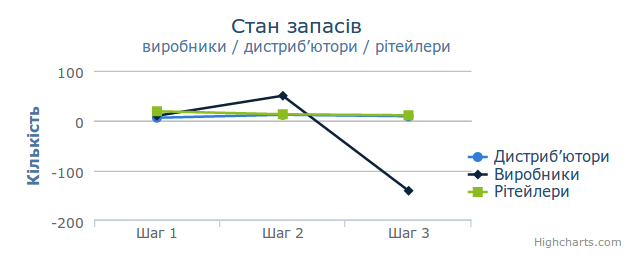
\includegraphics[width=4.5in]{images/plot.png}
    \caption{Стан запасів}
    \label{fig:plot}
\end{stdfigure}

